\chapter{Introduzione}
Con nucleo multiprogrammato intendiamo un sistema in grado di svolgere più \emph{processi}.
\begin{center}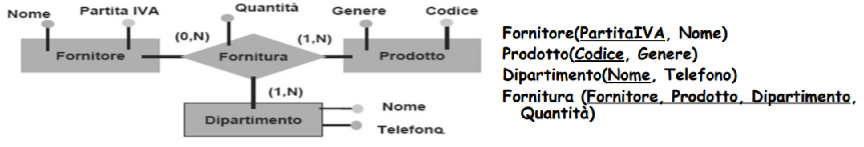
\includegraphics[scale=.80]{img/124.PNG}\end{center}
Il sistema che creiamo fornisce ai suoi utenti due astrazioni: \emph{processi} e \emph{primitiva}. Il meccanismo che realizza queste due astrazioni è detto \emph{contesto}.
\section{Concetti base}
\subsection{Processo} Il processo è \underline{un programma in esecuzione}. 
\[\text{Processo} \neq \text{Programma}\]
Pensiamo al pizzaiolo inesperto che sta facendo la pizza: ha bisogno di una ricetta, perché non si ricorda come si fa.
\begin{itemize}
	\item La ricetta è il programma, che posso utilizzare per creare le pizze (anche in contemporanea).
	\item Il pizzaiolo è il processore, la pizza i dati (l'input è la richiesta del cliente).
\end{itemize}
\textbf{Nessuna di queste cose è il processo}. Il processo possiamo immaginarlo come il filmato di tutto ciò che accade in questo sistema (\emph{pizza + pizzaiolo}), dall'inizio alla fine (il filmato di tutti gli stati attraverso cui il sistema passa).
\paragraph{Usciamo dalla metafora} Il processo è la sequenza degli stati attraverso cui passa il sistema eseguendo il programma. L'esecuzione di ogni istruzione del programma fa passare il processo da uno stato al successivo.
\paragraph{Programma vs Processo} Può essere facile confondere il processo col programma.
\begin{itemize}
	\item Un programma può essere eseguito da più processi "contemporaneamente". I clienti chiedono la pizza margherita, il pizzaiolo ne fa tante, ognuna di queste segue il suo processo indipendentemente dalle altre. 
	\item Un processo può eseguire programmi diversi. Si pensi alla \emph{pizza al metro}, con vari tipi di pizza uno dietro l'altro.
\end{itemize}
\paragraph{Fotogramma} 
\begin{itemize}
	\item Concentriamoci sul fotogramma: pur avendo una sequenza di stati possiamo concentrarci su uno stato in un particolare istante. \textbf{Per la natura dei nostri processi dato un qualunque fotogramma avrò le informazioni necessarie per proseguire il processo} (di ogni pizza il pizzaiolo si ricorda dove è arrivato).
	\item Passare da un processo a un altro significa ricordarsi il fotogramma dove è arrivato il processo da cui stiamo saltando via, caricarlo e spostarci sul fotogramma del nuovo processo che vogliamo portare avanti.
\end{itemize} Il processo è una cosa sequenziale. \textbf{Non possiamo, tuttavia, definire il processo come l'istanza di un programma}: un processo, ricordiamolo, può cambiare programma. 
\begin{itemize}
	\item  Il programma non è la sceneggiatura del processo: la ricetta può contenere delle varianti (quattro stagioni con o senza carciofi...). Il processo di produzione di una singola pizza riguarda una sola delle varianti possibili.
	\item Il programma potrebbe contenere dei cicli. Nel programma vediamo le azioni ripetute una volta sola, mentre nel processo vediamo le azioni effettivamente ripetute tante volte.
\end{itemize}

\subsection{Primitiva}
\paragraph{Cosa intendiamo con \emph{primitivo}} Primitivo è un qualcosa di \textit{non derivato}, un mattone fornito dal sistema per costruire il resto delle cose. L'esempio sono le funzionalità di base fornite da un programma di grafica. Ricordarsi la caratteristica fondamentale delle primitive:
\[\boxed{\text{La primitiva non è scomponibile.}}\]
\paragraph{Funzioni di libreria?} Si potrebbe dire che le primitive sono funzioni di libreria non scomponibili (di solito lo sono).
\paragraph{Tipi primitivi} I tipi primitivi di un linguaggio (int, long, char...) sono offerti dal linguaggio, possono essere usati per definire nuovi tipi derivati, ma non possono essere modificati nel comportamento.

\paragraph{Cosa faremo a breve} Creeremo un sistema che fornisce una stazione dei processi, esegue programmi all'interno dei processi, fornisce delle primitive che sono le funzionalità di base presenti all'interno di questi programmi.
\begin{itemize}
	\item Gli utenti possono lanciare le primitive e usufruire dei servizi da esse offerte.
	\item Normalmente le primitive di un sistema sono pensate come {chiamate di sistema}, dunque con privilegio maggiore. Le primitive molto spesso reggono il loro funzionamento su delle strutture dati: queste strutture dati non devono essere manipolabili dall'utente, o al più manipolabili in modo controllato (non raggiungibili dal livello utente se non attraverso una primitiva).
	\item Gli utenti non possono manipolare le primitive esistenti, ma soprattutto non possono crearne di nuove.
\end{itemize}

\subsection{Contesto}
Con la parola contesto si intende, nel linguaggio comune, tutto ciò che è necessario sapere per interpretare correttamente un dato testo, ma che non è scritto esplicitamente nel testo stesso. Prendiamo ad esempio la seguente istruzione C++:
\begin{verbatim}
	x = x + 1
\end{verbatim}
abbiamo una somma, ma non sappiamo in cosa consista \emph{x}.

\paragraph{E nel nostro caso?} Il contesto permette la realizzazione delle astrazioni \emph{processo} e \emph{primitiva}. Se io ho più processi che vanno avanti, anche processi che eseguono lo stesso programma, avrò per ciascuno uno stato. (i registri relativi a un processo potrebbero non essere i registri relativi a un altro processo). \textbf{In un certo senso il \emph{contesto} consiste nello stato del processo}. Associo un contesto diverso ad ogni processo (nel nucleo faremo ciò con un \emph{descrittore di processo}).
\paragraph{Cambio di contesto}
Quando si passa da un processo a un altro si dice che \emph{si cambia contesto}. Il processore, chiaramente, può dedicarsi a un solo processo alla volta: l'unico modo per avere un'esecuzione apparentemente concorrente dei processi è eseguire in modo frammentato i processi (eseguo un pezzo di un processo, cambio contesto, eseguo un pezzo di un altro processo, cambio nuovamente contesto, e così via...)
\paragraph{Contesto e primitive}
Questa idea di contesto è valida anche per le primitive: supponiamo di avere un'istruzione HLT, è lecito o non è lecito eseguirla? Di per sè non è nè lecita, nè illecita. Dipende solo da chi la vuole eseguire: un utente non ne ha diritto, il sistema sì. Anche l'invocazione di primitiva da parte di un processo può essere immaginato come un \emph{cambio di contesto} (meno drammatico rispetto al cambio di contesto vero e proprio), che definiamo \emph{cambio di privilegio} per distinguerlo dai cambi di processo.

\section{Moduli} Il sistema che andiamo a studiare è realizzato in moduli: ogni modulo è un programma a se stante eseguito in un contesto (di privilegio) diverso. 
\begin{itemize}
	\item Il \textbf{modulo sistema} deve essere eseguito a livello sistema;
	\item Il \textbf{modulo I/O} è eseguito a livello sistema (la soluzione ideale sarebbe eseguirlo a un livello di privilegio intermedio, ma abbiamo solo due modalità - sistema e utente);
	\item Il \textbf{modulo utente} è eseguito a livello utente. 
\end{itemize}
In sostanza...
\begin{itemize}
	\item Il programmatore di sistema scrive delle primitive, che svolgono operazioni per conto dell'utente (impedisco all'utente di occuparsi delle periferiche, ad esempio, ma gli dico che posso farlo io). Il codice di sistema, così come le primitive e le strutture dati su cui si reggono, sono posti nel modulo sistema e nel modulo I/O (vedremo verso la fine l'utilità del modulo I/O). 
	\item Le primitive possono essere invocate esclusivamente passando da un gate della IDT, innalzando il livello del processore.  
	\item L'utente si scrive i programmi di cui ha bisogno e li esegue in modalità utente, facendo eventuale ricorso alle primitive offerte dal nucleo. 
\end{itemize} Il modulo sistema e il modulo I/O costituiscono, di fatto, un sistema operativo non modificato dall'utente, che riceve il programma e lo esegue.

\section{Cartelle}
\paragraph{Modulo sistema} I file che compongono il modulo sistema stanno nella directory 
\begin{verbatim}sistema\end{verbatim}
tutto è posto in due file: \emph{sistema.cpp} (parte C++) e \emph{sistema.s} (parte Assembler). 

\paragraph{Modulo I/O} I file che compongono il modulo I/O stanno nella directory
\begin{verbatim}io\end{verbatim}
anche in questo caso abbiamo tutto in due file: \emph{io.cpp} (parte C++) ed \emph{io.s} (parte Assembler).

\paragraph{Modulo utente} I file che compongono il modulo utente stanno nella directory
\begin{verbatim}utente\end{verbatim}
abbiamo più files: 
\begin{itemize}
	\item \emph{all.h}
	\item \emph{lib.cpp}
	\item \emph{lib.h}
	\item \emph{utente.s}
	\item \emph{utente.cpp}
\end{itemize}
La cosa è necessaria per permettere all'utente di scrivere solo la parte che gli interessa (quella C++, nell'ultimo file). 

\paragraph{Approccio} L'approccio è il solito: utilizzare Linux come sistema di appoggio per \emph{cross-compiling}.  Compiliamo su Linux programmi pensati per girare come sistema. 

\section{Esempio di scrittura del file \emph{utente.cpp}:  Hello, world!}
\small
\begin{verbatim}
	#include <all.h>
	
	void main() {
		writeconsole("Hello, world!\n", 14);
		pause(); /* Per evitare che il processo venga terminato subito */
		terminate_p();
	}
\end{verbatim}
\normalsize
\begin{itemize}
	\item Includiamo \emph{all.h} per avere a disposizione tutte le funzioni.
	\begin{verbatim}
		#include <costanti.h>
		#include <libce.h>
		#include <sys.h>
		#include <io.h>
		#include "lib.h"
	\end{verbatim}
	\item Scriviamo il \emph{main}, che non è standard (attenzione al \emph{void}). Il sistema lo esegue all'interno di un processo: quando il processo termine e non ci sono altre cose da fare il sistema spegne la macchina.
	\item Un esempio di primitiva è \emph{writeconsole}
	\begin{verbatim}
		writeconsole("Hello, world!\n", 14);
	\end{verbatim}
	passiamo la stringa e indichiamo la sua lunghezza.
	\item \emph{terminate$\_$p} è un altro esempio di primitiva, invocata per terminare esplicitamente il processo.
	\item Si osservi che entrambe le primitive comportano un cambio di privilegio: la prima sarà eseguita dal modulo I/O (poichè posta nel modulo I/O), la seconda dal modulo sistema (poichè posta nel modulo sistema).
\end{itemize}
%\section{tbd}
%Il processore Intel si fa tutta la storia dei processori Intel dall'8086 all'AMD64, cioè parte in una modalità sostanzialmente compatibile con l'8086 (a 16 bit, senza protezione), attraverso dei registri di controllo passa a una modalità compatibile col 386 (a 32 bit), e infine si pone in una modalità compatibile con l'AMD64 (a 64 bit). I programmi da noi scritti (e il modulo sistema) partono suppendo che il processore sia già nell'ultima modalità dunque il bootloader deve portarci in questa modalità (il primo passaggio a 32 bit se ne occupa QEMU, quello da 32 bit a 64 bit lo fa il bootloader). A questo punto vengono posti in memoria i segmenti del file ELF \emph{sistema}, e cede il controllo. Il file ELF \emph{sistema}, dopo essere stato caricato, interpreta gli altri due file rimanenti (\emph{IO} e \emph{utente}): questa cosa deve farla per forza lui.
\section{Compilazione e avvio del sistema}
Eseguiamo il comando \emph{make} nella root
\begin{verbatim}
	make
\end{verbatim}
la procedura ha creato, nella cartella \emph{build} tre file ELF: modulo utente, modulo sistema e modulo I/O. Ribadiamo che ciò che abbiamo ottenuto non è pensato per essere eseguito su Linux ma su un'altra macchina avente architettura comune.


\paragraph{Avvio del sistema}
\begin{itemize}
	\item Il modulo sistema è il primo modulo caricato dal bootloader. Il modulo sistema questa volta è un po' più sofisticato: inizializza le sue strutture dati, prepara i moduli I/O e utente. Il bootloader si limita solo a caricare questi moduli in memoria, il modulo sistema li interpreta. Quando è tutto pronto viene creato un nuovo processo e si avvia l'esecuzione del programma \emph{main} in quel processo, a livello utente. 
	\item Osserviamo che all'avvio viene inizializzata la GDT (accompagnata da alcuni elementi della segmentazione necessari per definire i livelli di privilegio), l'APIC, il timer (che restituisce periodicamente il controllo al sistema). il modulo IO con tutte le periferiche che conosciamo (tastiera, video, busmaster). Dopo tutte queste inizializzazioni passo il controllo all'utente.
	\item Ogni processo è identificato da un numero, visibile nel terminale (dei vari messaggi e warning si vede il relativo processo) .
	\item Il processore esegue il sistema o il modulo utente. Risponde a tutte le chiamate di sistema che l'utente potrebbe fare, e a tutte le eccezioni/interruzioni, che provocano la restituzione del controllo al modulo sistema (o al modulo I/O in alcuni casi).
\end{itemize}

\section{Esempio di programma bloccato dalla protezione}
\small
\begin{verbatim}
	#include <all.h>
	
	void main() {
		volatile natw* video = (natw*)0xb8000;
		video[4] = 0x3F00 | `a';
		
		pause(); /* Per evitare che il processo venga terminato subito */
		terminate_p();
	}
\end{verbatim}
\normalsize
\begin{itemize}
	\item Proviamo a scrivere in memoria video senza utilizzare la primitiva \emph{writeconsole}.
	\item Se compiliamo non succede nulla, ma quando avvieremo il sistema il nostro programma verrà interrotto. Nel momento in cui ha provato a scrivere in quella zona di memoria il processore si è rifiutato e ha lanciato un'eccezione 14 di \emph{page fault}: il controllo è stato restituito al sistema, la routine andata in esecuzione ha interrotto il processo e stampato una miriade di informazioni (che dovrebbero aiutarci a capire in che stato si trovava il processo al momento dell'errore).
	\begin{center}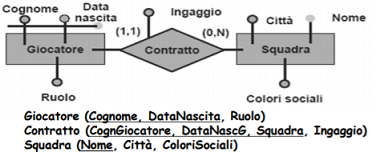
\includegraphics[scale=.85]{img/125.PNG}\end{center}
	Vediamo che l'eccezione è stata provocata da una certa riga di \emph{utente.cpp}, vediamo anche l'indirizzo di memoria relativo. Si indica il livello di privilegi corrente al momento di esecuzione dell'istruzione, i valori dei registri (RFLAGS, IF, IOPL, RAX, RBX...). Per quanto riguarda il registro RIP il log è automaticamente decodificato, se l'indirizzo è associabile a una riga del sorgente si pone direttamente il numero di riga. Possiamo evitare questa cosa nel seguente modo
	\begin{verbatim}
		CERAW=1 ./run
	\end{verbatim}
\end{itemize}

\subsection{\emph{backtrace}} Il backtrace mostra lo stack delle chiamate. Proviamo a porre il programmino precedente nel seguente modo:
\small
\begin{verbatim}
	#include <all.h>
	void f1() {
		volatile natw* video = (natw*)0xb8000;
		video[4] = 0x3F00 | `a';
	}
	
	void f2() { f1(); }
	
	void main() {
		f2();
		pause(); /* Per evitare che il processo venga terminato subito */
		terminate_p();
	}
\end{verbatim}
\normalsize
Otteniamo un lancio di eccezione anche in questo caso
\begin{center}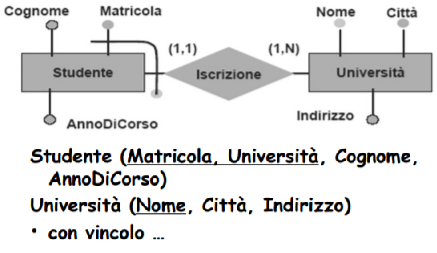
\includegraphics[scale=.85]{img/126.PNG}\end{center}
\begin{itemize}
	\item Si specifica che al momento dell'errore l'instruction pointer era dentro \emph{f1}.
	\item Si indica che \emph{f2} è stata chiamata da \emph{f1},  a sua volta chiamata da \emph{main}. In entrambi i casi si indica la riga del sorgente con la chiamata. 
\end{itemize}
Il backtrace è utile perché la funzione potrebbe essere chiamabile da più punti del nostro sorgente.

\section{Libreria \emph{libce}}
\small
\begin{verbatim}
	#include <all.h>
	
	void f1() {
		char_write(`a');
	}
	
	void f2() { 
		f1(); 
	}
	
	void main() {
		f2();
		pause(); /* Per evitare che il processo venga terminato subito */
		terminate_p();
	}
\end{verbatim}
\normalsize
Il nostro programma è collegato anche con la libreria \emph{libce}, stessa cosa il modulo I/O. Per scrivere su video i codici da scrivere sono i soliti già visti. Dobbiamo ricordarci che non è il codice a dirci il livello di privilegio, ma il contesto.